\section{
  Dusty vertical shear instability}\label{results} 

When $\tstop=0$ we may construct exact dusty equilibra by specifying
the dust-to-gas ratio, as described in \S\ref{eqm}. We use this to
examine the effect of dust on classic VSI, defined to be driven by the
temperature gradient (\S\ref{dusty_vsi_int}). For simplicity we
consider constant input values of the midplane dust-to-gas ratio
$\epsilon_0$ and the characteristic dust thickness $\Hd$. These,
together with the perturbation wavenumber $k$, comprises main the
parameters of the linear problem. We fix the radial power-law index
for the midplane gas density to $p = -1.5$, that for the
temperature profile to $q=-1$; and set the gas disk aspect-ratio
$h_\mathrm{g}=0.05$. These are fiducial values used in \citetalias{lin15}. 

\subsection{Effect of dust-loading}
We first vary the dust-to-gas ratio $\epsilon_0\in[10^{-3},1]$,
fixing the dust thickness to $\Hd=0.99\Hg$ (so that $\epsilon$ is
roughly constant with height) and perturbation
wavenumber to $k\Hg = 30$. 

Fig. \ref{vsi_dust_loading} show unstable
modes for different values of $\epsilon_0$. The eigenvalue
distributions for $\epsilon_0 \leq 10^{-2}$ are similar to the
dust-free fiducial case considered by \citetalias{lin15}, consisting
of the roughly horizontal `body modes' and the nearly-vertical
`surface modes'. The latter is due to the imposed vertical boundaries
\citep{barker15}.  

We find that increasing the dust-to-gas ratio reduce VSI growth
rates. Notably `surface modes', which are typically fastest growing in
the dust-free case, are surpressed in dusty disks for $\epsilon_0\geq
0.1$. The body modes' growth rates remain $\sim O(h_\mathrm{g}\OmK)$
but their oscillation frequency increases with
$\epsilon_0$. The total number of modes do not change
significantly. This is in contrast with the effect of increasing
cooling times, where \citetalias{lin15} find fewer unstable modes.
%until the system is eventually completely stable. 

\begin{figure}
  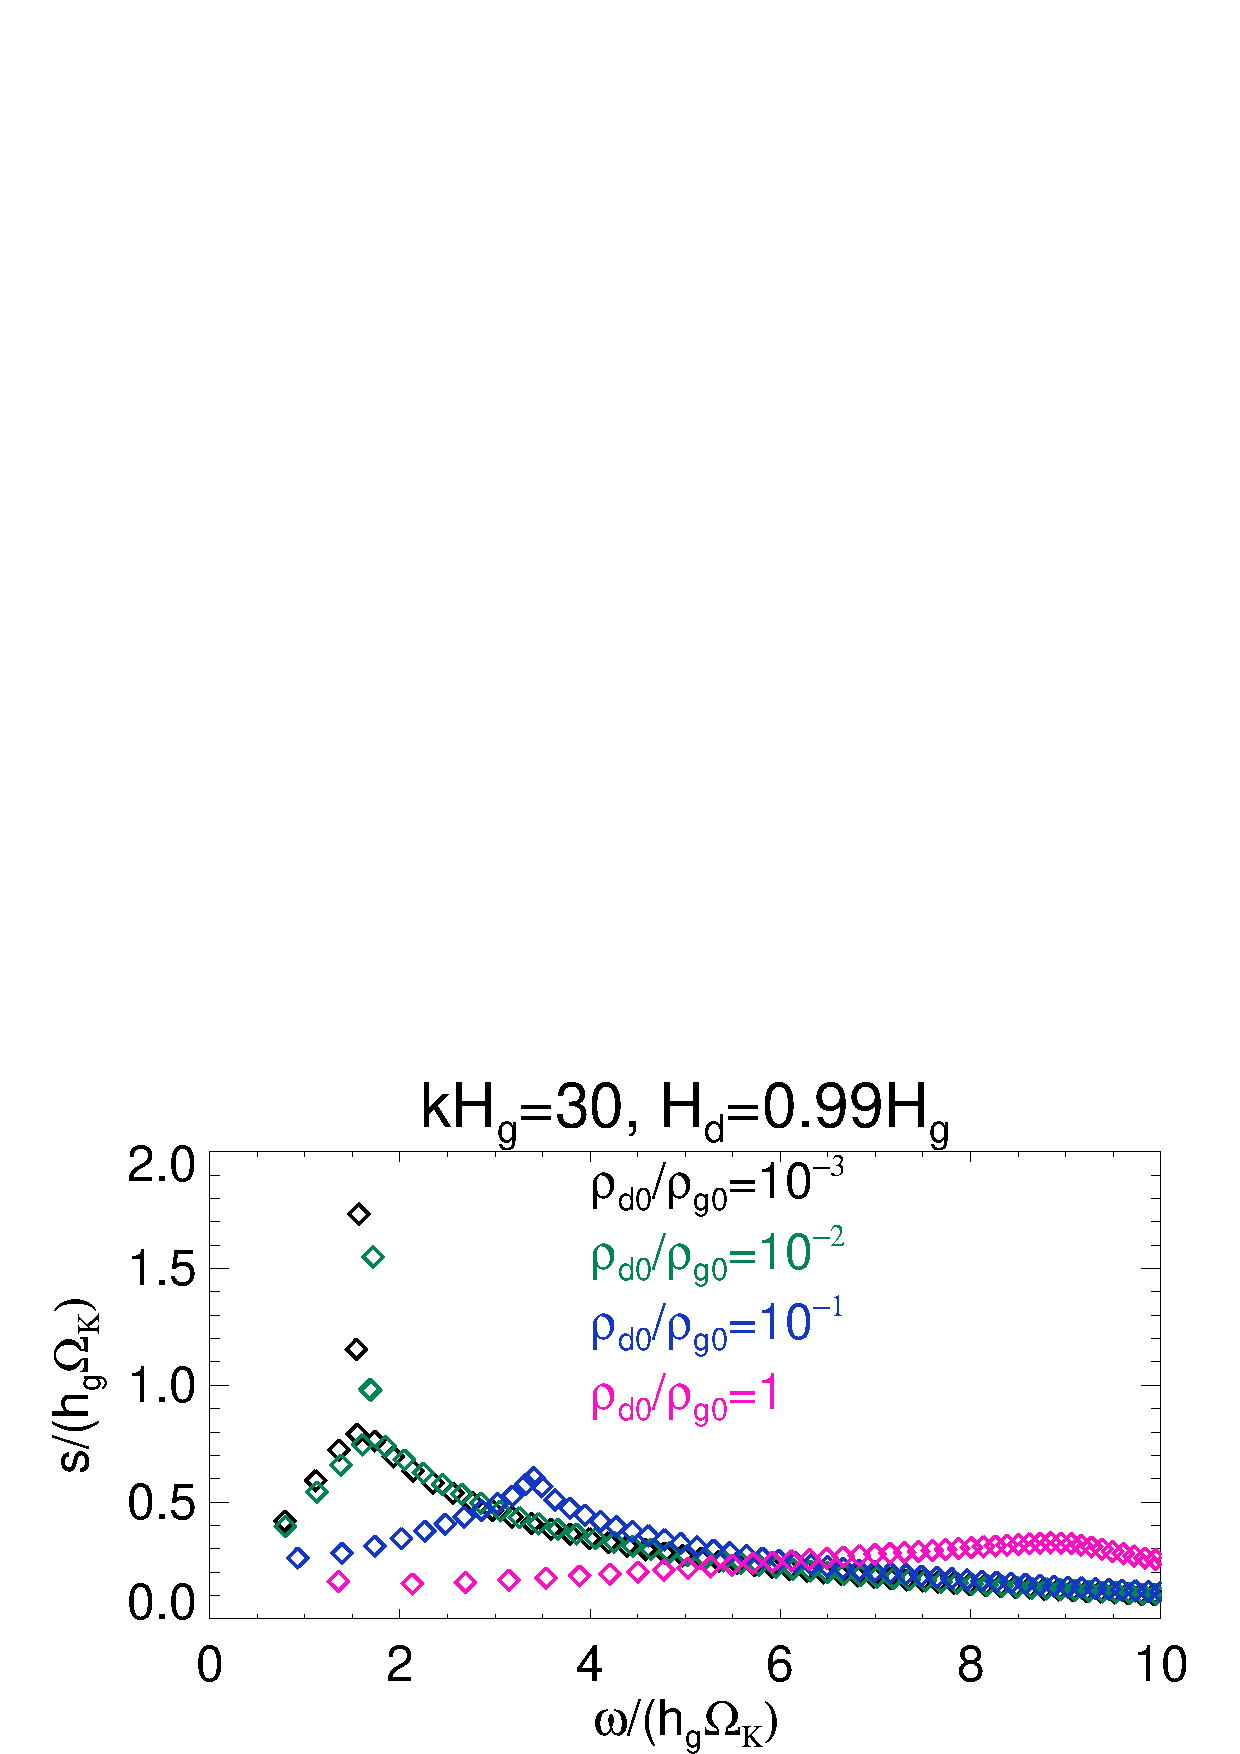
\includegraphics[width=\linewidth]{figures/compare_eigenvals_kx30Hd1} 
  \caption{Unstable modes in a locally isothermal, perfectly coupled
    dusty disk with fiducial parameters
    $(p,q,h_\mathrm{g}, \Hd/\Hg )=(-1.5,-1,0.05, 0.99)$. The real
    frequency $\omega$ and growth rates $s$ are shown for a range of
    midplane dust-to-gas ratios $\epsilon_0=\rho_\mathrm{g0}/\rho_\mathrm{d0}$. 
    \label{vsi_dust_loading}
    }
\end{figure}

The lowest frequency `fundamental' body mode is not the fastest
growing, but they are energetically dominant because the entire disk
column is perturbed \citep[cf. surface modes which only disturb the
  disk boundaries,][]{umurhan16c}. In Fig. \ref{vsi_dust_loading2d}
we compare the fundamental mode between the nearly 
dust-free case $\epsilon_0=10^{-3}$ an a dusty disk with
$\epsilon_0=1$. Dust-loading preferentially
stabilizes the disk atmosphere against the VSI, restricting
meridional motions to $|z|\lesssim 2\Hg$, where most of the disk mass
reside. Notice also the perturbed dust-to-gas ratio,
$\delta\epsilon$, shifts from being maximized at the disk boundaries
to the midplane. 

\begin{figure}
  \includegraphics[scale=0.54, clip=true, trim=0cm 2.5cm 0cm 0cm]{figures/result2d_dg1d-3.ps}\\
  \includegraphics[scale=0.54]{figures/result2d_dg1.ps} 
  \caption{Fundamental dusty VSI mode in real space for midplane dust-to-gas
    ratio $\epsilon_0=10^{-3}$ (top) and $\epsilon_0=1$
    (bottom). The color scale shows the perturbation to the
    dust-to-gas ratio, $\delta\epsilon$; and the arrows show
    $\sqrt{\rho}\left(\dd v_x, \dd v_z\right)$. 
    \label{vsi_dust_loading2d}
    }
\end{figure}






In Fig. \ref{vsi_dust_loading_vareps} we plot the growth rates as a
function of $\epsilon_0$ for different perturbation wavenumbers $k$. We
find that dust-loading stabilizes the VSI more effectively for shorter
wavelength perturbations. This is because for high wavenumbers the
dominant modes are surface modes, which are stabilized by
dust-loading. The figure suggest that VSI becomes much less efficient
for $\epsilon_0\gtrsim 0.1$ and $k\Hg\gtrsim 50$. 

\begin{figure}
  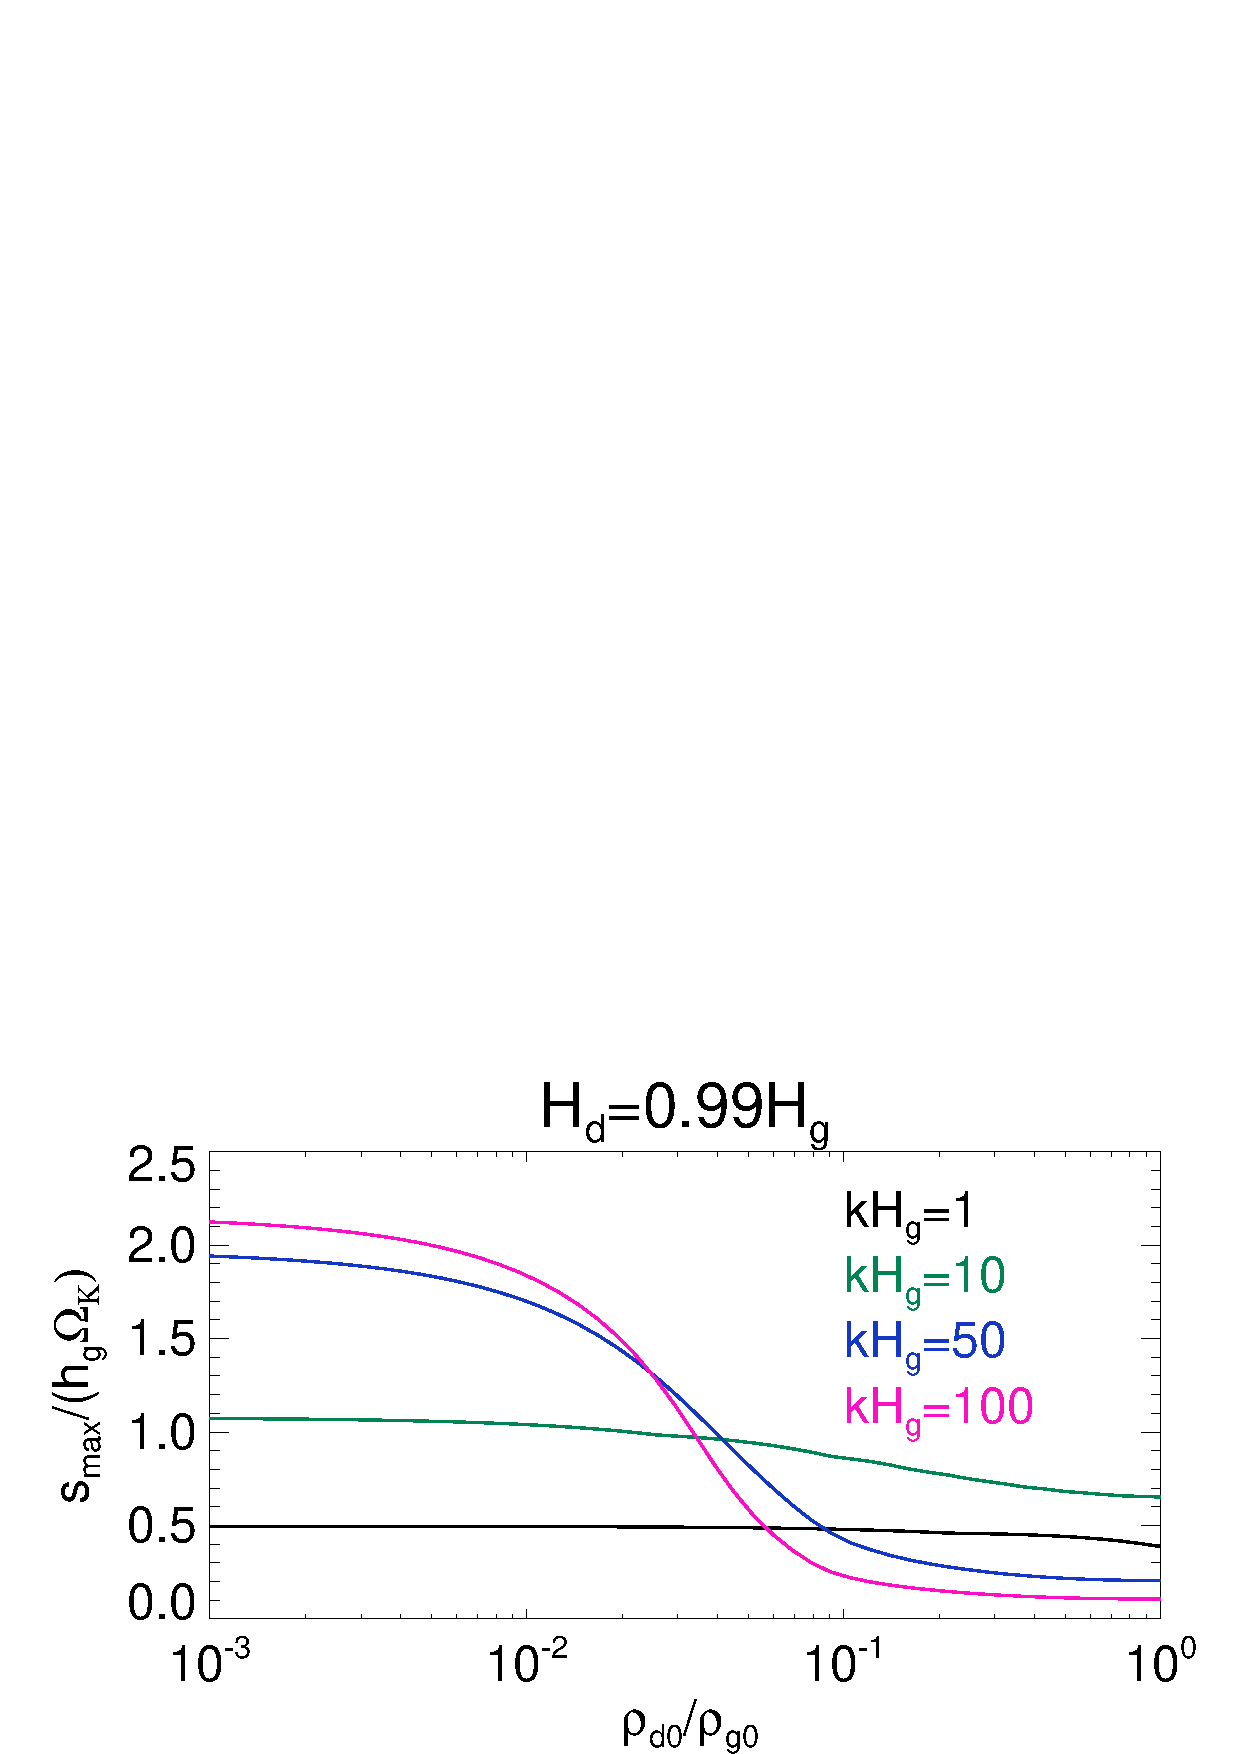
\includegraphics[width=\linewidth]{figures/compare_eigenvals_vareps} 
  \caption{Maximum growth rate of the dusty VSI as a function of the
    midplane dust-to-gas ratio $\epsilon_0$ for perturbations with
    different radial wavenumbers $k$. The dust layer thickness is
    fixed to $\Hd\simeq \Hg$. 
    \label{vsi_dust_loading_vareps}
    }
\end{figure}

\subsection{Effect of dust thickness}



\subsection{Fixed metalicity} 
Here we vary the dust layer thickness $\Hd$ but hold 
\begin{align}\label{metalicity_def}
Z \equiv \epsilon_0 \Htilde = \text{constant,}
\end{align}
so that $\Sigma_\mathrm{d}/\Sigma_\mathrm{g}$ is
fixed. Eq. \ref{metalicity_def} then gives the required midplane
dust-to-gas ratio. 

%zmax = 2 because we have very thin dust layer

We set $Z=0.03$ and consider two disks with $\Hd=0.1\Hg$ and
$\Hd=0.99\Hg$. Fig. \ref{compare_vshear_fixZ} compares the 

\begin{figure}
  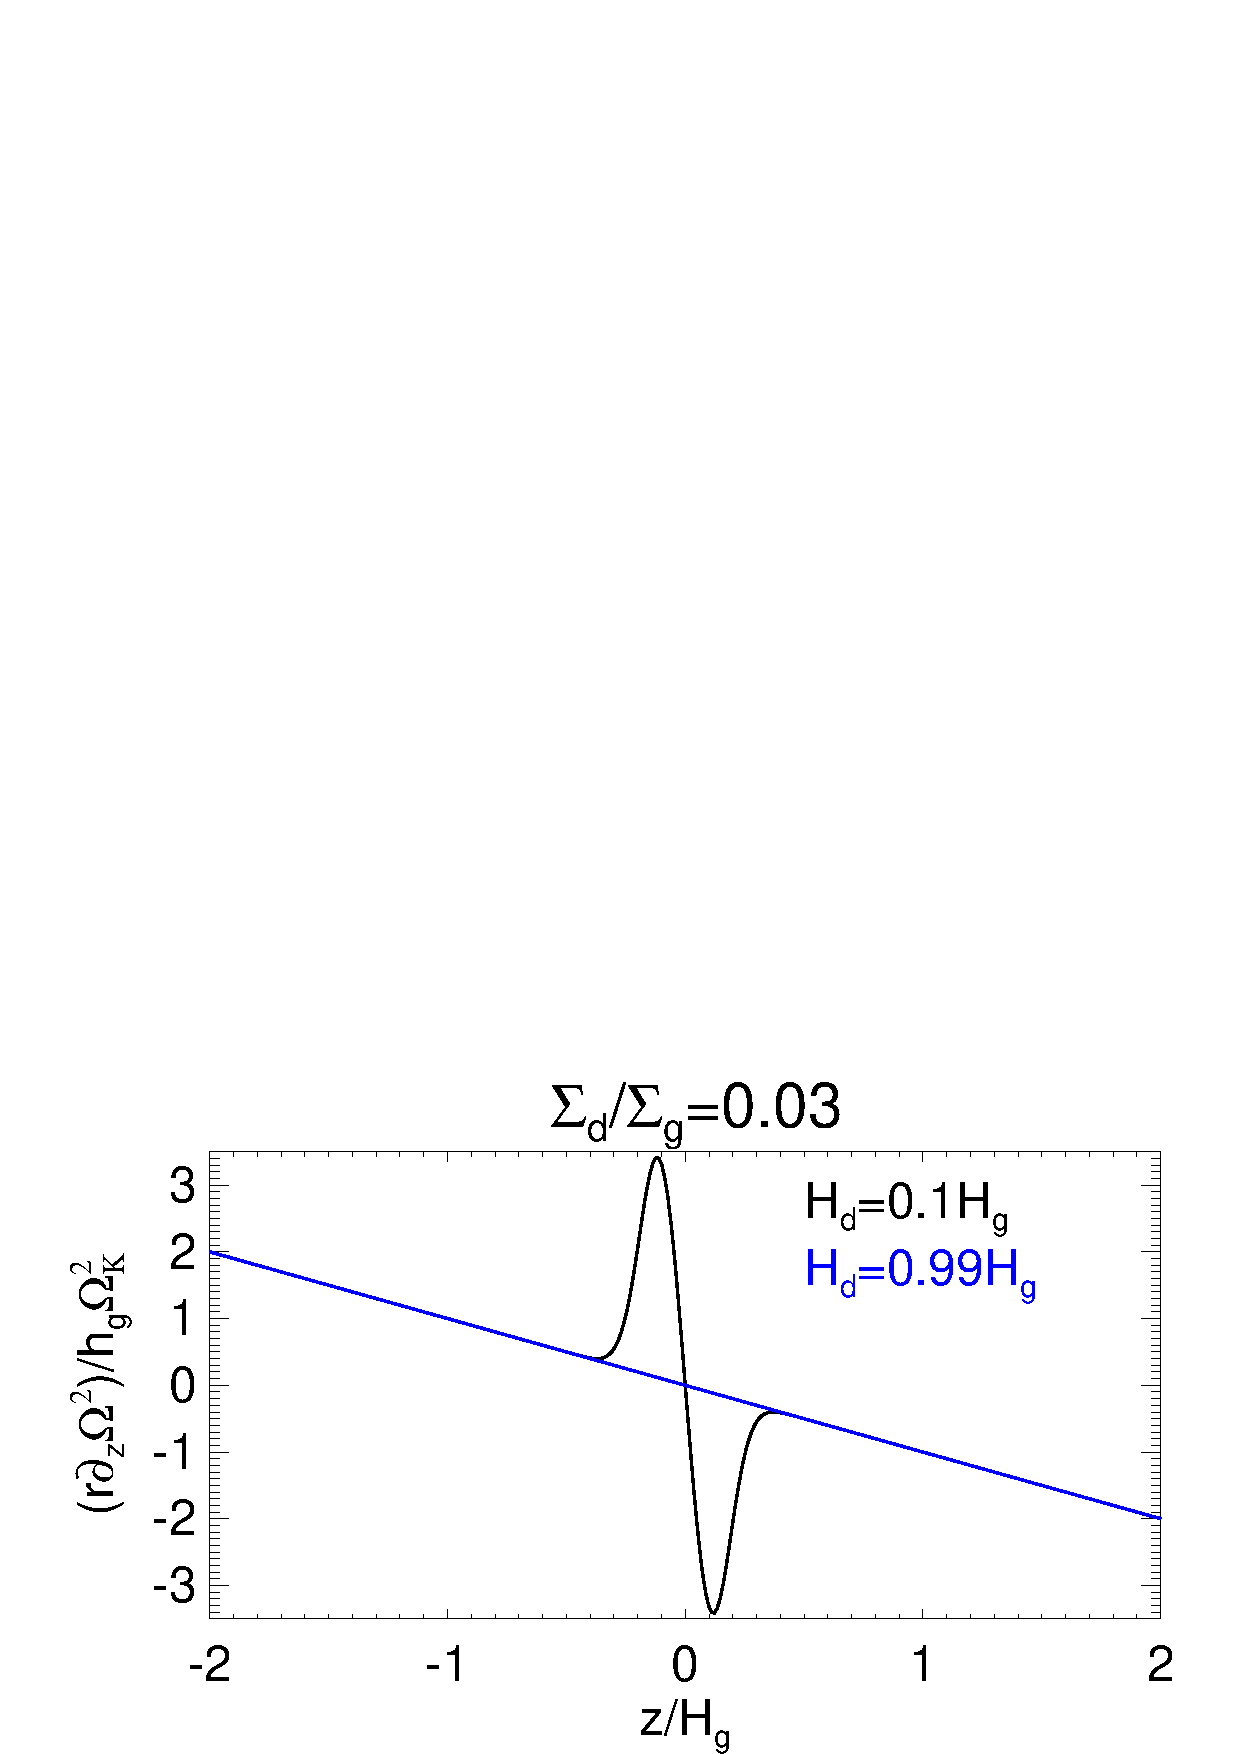
\includegraphics[width=\linewidth]{figures/compare_vshear_fixZ} 
  \caption{Vertical shear rate in a locally isothermal, dusty disk
    with fixed dust-to-gas mass and dust thickness $\Hd=0.1\Hg$
    (black) and $\Hd=0.99\Hg$ (blue). 
    \label{compare_vshear_fixZ}
    }
\end{figure}



\begin{figure}
  \includegraphics[scale=0.33, clip=true, trim=0.5cm 0cm 3cm 0cm]{figures/result2d_Hd1.ps}\includegraphics[scale=0.33, clip=true, trim=2cm 0cm 0cm 0cm]{figures/result2d_Hd0d1.ps} 
  \caption{
%dusty VSI mode in real space for midplane dust-to-gas
%    ratio $\epsilon_0=10^{-3}$ (top) and $\epsilon_0=1$
%    (bottom). The color scale shows the perturbation to the
%    dust-to-gas ratio, $\delta\epsilon$; and the arrows show
%    $\sqrt{\rho}\left(\dd v_x, \dd v_z\right)$. 
    stuff
    \label{result2d_fixZ}
    }
\end{figure}
